% Fig 4: Design lever taxonomy matrix
% Seven strategies x five columns; explicit node placement to avoid foreach-tuple errors.
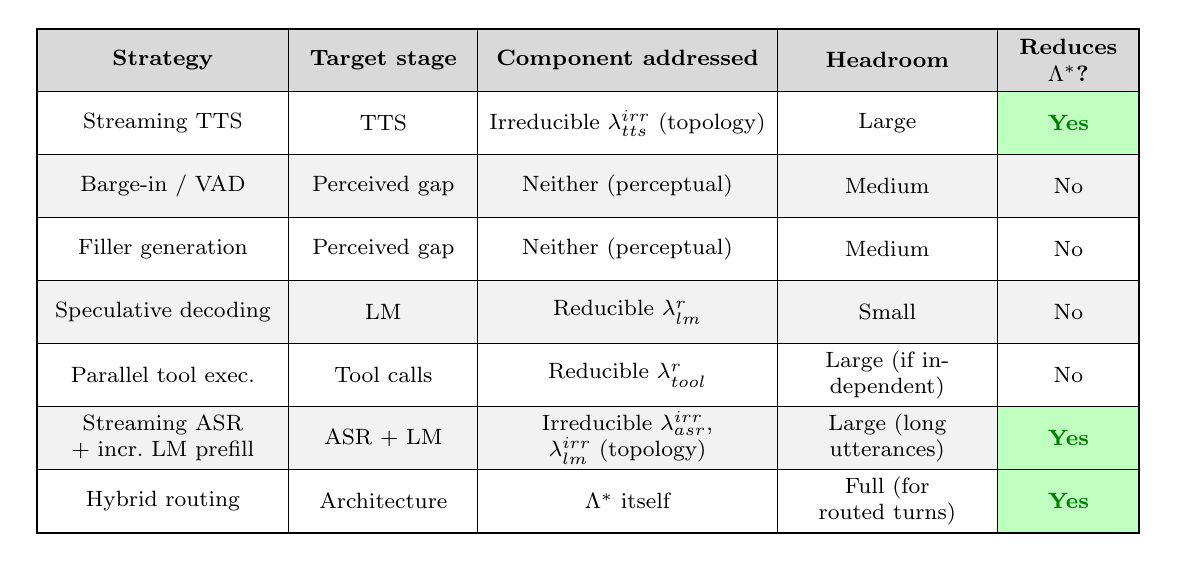
\begin{tikzpicture}[font=\footnotesize]

% Geometry (unitless numbers; appended with "cm" at each use)
\def\rh{0.80}  % row height (cm)
\def\ca{3.2}   % col 1 width: Strategy
\def\cb{2.4}   % col 2 width: Target stage
\def\cc{3.8}   % col 3 width: Component addressed
\def\cd{2.8}   % col 4 width: Headroom
\def\ce{1.8}   % col 5 width: Reduces Lambda*?

% Derived x-positions of left edges of each column
\pgfmathsetmacro{\xA}{0}
\pgfmathsetmacro{\xB}{\xA+\ca}
\pgfmathsetmacro{\xC}{\xB+\cb}
\pgfmathsetmacro{\xD}{\xC+\cc}
\pgfmathsetmacro{\xE}{\xD+\cd}
\pgfmathsetmacro{\xF}{\xE+\ce}

% Derived x-positions of centres of each column
\pgfmathsetmacro{\mA}{\xA+\ca/2}
\pgfmathsetmacro{\mB}{\xB+\cb/2}
\pgfmathsetmacro{\mC}{\xC+\cc/2}
\pgfmathsetmacro{\mD}{\xD+\cd/2}
\pgfmathsetmacro{\mE}{\xE+\ce/2}

% ── HEADER ROW (y = 0 to +\rh) ──────────────────────────────────────────────
\fill[gray!30] (\xA,0) rectangle (\xF,\rh);
\node[align=center, font=\footnotesize\bfseries, text width=\ca cm] at (\mA,{0.5*\rh}) {Strategy};
\node[align=center, font=\footnotesize\bfseries, text width=\cb cm] at (\mB,{0.5*\rh}) {Target stage};
\node[align=center, font=\footnotesize\bfseries, text width=\cc cm]
  at (\mC,{0.5*\rh}) {Component addressed};
\node[align=center, font=\footnotesize\bfseries, text width=\cd cm] at (\mD,{0.5*\rh}) {Headroom};
\node[align=center, font=\footnotesize\bfseries, text width=\ce cm]
  at (\mE,{0.5*\rh}) {Reduces $\Lambda^*$?};

% ── Helper macro: row shading ────────────────────────────────────────────────
% Row 1: y from 0 down to -\rh, row 2: -\rh to -2*\rh, etc.

% Row 1 — Streaming TTS (YES — highlighted green for last cell)
\fill[white]     (\xA,{-0*\rh}) rectangle (\xF,{-1*\rh});
\fill[green!25]  (\xE,{-0*\rh}) rectangle (\xF,{-1*\rh});
\node[align=center, text width=\ca cm]
  at (\mA,{-0.5*\rh}) {Streaming TTS};
\node[align=center, text width=\cb cm]
  at (\mB,{-0.5*\rh}) {TTS};
\node[align=center, text width=\cc cm]
  at (\mC,{-0.5*\rh}) {Irreducible $\lambda_{tts}^{irr}$ (topology)};
\node[align=center, text width=\cd cm]
  at (\mD,{-0.5*\rh}) {Large};
\node[align=center, font=\footnotesize\bfseries, color=green!50!black, text width=\ce cm]
  at (\mE,{-0.5*\rh}) {Yes};

% Row 2 — Barge-in / VAD
\fill[gray!10]   (\xA,{-1*\rh}) rectangle (\xF,{-2*\rh});
\node[align=center, text width=\ca cm]
  at (\mA,{-1.5*\rh}) {Barge-in / VAD};
\node[align=center, text width=\cb cm]
  at (\mB,{-1.5*\rh}) {Perceived gap};
\node[align=center, text width=\cc cm]
  at (\mC,{-1.5*\rh}) {Neither (perceptual)};
\node[align=center, text width=\cd cm]
  at (\mD,{-1.5*\rh}) {Medium};
\node[align=center, text width=\ce cm]
  at (\mE,{-1.5*\rh}) {No};

% Row 3 — Filler generation
\fill[white]     (\xA,{-2*\rh}) rectangle (\xF,{-3*\rh});
\node[align=center, text width=\ca cm]
  at (\mA,{-2.5*\rh}) {Filler generation};
\node[align=center, text width=\cb cm]
  at (\mB,{-2.5*\rh}) {Perceived gap};
\node[align=center, text width=\cc cm]
  at (\mC,{-2.5*\rh}) {Neither (perceptual)};
\node[align=center, text width=\cd cm]
  at (\mD,{-2.5*\rh}) {Medium};
\node[align=center, text width=\ce cm]
  at (\mE,{-2.5*\rh}) {No};

% Row 4 — Speculative decoding
\fill[gray!10]   (\xA,{-3*\rh}) rectangle (\xF,{-4*\rh});
\node[align=center, text width=\ca cm]
  at (\mA,{-3.5*\rh}) {Speculative decoding};
\node[align=center, text width=\cb cm]
  at (\mB,{-3.5*\rh}) {LM};
\node[align=center, text width=\cc cm]
  at (\mC,{-3.5*\rh}) {Reducible $\lambda_{lm}^r$};
\node[align=center, text width=\cd cm]
  at (\mD,{-3.5*\rh}) {Small};
\node[align=center, text width=\ce cm]
  at (\mE,{-3.5*\rh}) {No};

% Row 5 — Parallel tool execution
\fill[white]     (\xA,{-4*\rh}) rectangle (\xF,{-5*\rh});
\node[align=center, text width=\ca cm]
  at (\mA,{-4.5*\rh}) {Parallel tool exec.};
\node[align=center, text width=\cb cm]
  at (\mB,{-4.5*\rh}) {Tool calls};
\node[align=center, text width=\cc cm]
  at (\mC,{-4.5*\rh}) {Reducible $\lambda_{tool}^r$};
\node[align=center, text width=\cd cm]
  at (\mD,{-4.5*\rh}) {Large (if independent)};
\node[align=center, text width=\ce cm]
  at (\mE,{-4.5*\rh}) {No};

% Row 6 — Streaming ASR + Incremental LM prefill (YES — highlighted green)
\fill[gray!10]   (\xA,{-5*\rh}) rectangle (\xF,{-6*\rh});
\fill[green!25]  (\xE,{-5*\rh}) rectangle (\xF,{-6*\rh});
\node[align=center, text width=\ca cm]
  at (\mA,{-5.5*\rh}) {Streaming ASR + incr.\ LM prefill};
\node[align=center, text width=\cb cm]
  at (\mB,{-5.5*\rh}) {ASR + LM};
\node[align=center, text width=\cc cm]
  at (\mC,{-5.5*\rh}) {Irreducible $\lambda_{asr}^{irr}$, $\lambda_{lm}^{irr}$ (topology)};
\node[align=center, text width=\cd cm]
  at (\mD,{-5.5*\rh}) {Large (long utterances)};
\node[align=center, font=\footnotesize\bfseries, color=green!50!black, text width=\ce cm]
  at (\mE,{-5.5*\rh}) {Yes};

% Row 7 — Hybrid routing (YES — highlighted green)
\fill[white]     (\xA,{-6*\rh}) rectangle (\xF,{-7*\rh});
\fill[green!25]  (\xE,{-6*\rh}) rectangle (\xF,{-7*\rh});
\node[align=center, text width=\ca cm]
  at (\mA,{-6.5*\rh}) {Hybrid routing};
\node[align=center, text width=\cb cm]
  at (\mB,{-6.5*\rh}) {Architecture};
\node[align=center, text width=\cc cm]
  at (\mC,{-6.5*\rh}) {$\Lambda^*$ itself};
\node[align=center, text width=\cd cm]
  at (\mD,{-6.5*\rh}) {Full (for routed turns)};
\node[align=center, font=\footnotesize\bfseries, color=green!50!black, text width=\ce cm]
  at (\mE,{-6.5*\rh}) {Yes};

% ── GRID LINES ───────────────────────────────────────────────────────────────

% Outer border
\draw[thick] (\xA,\rh) rectangle (\xF,{-7*\rh});

% Horizontal row separators (between header and row 1, and between data rows)
\foreach \row in {0,1,2,3,4,5,6} {
  \draw (\xA,{-\row*\rh}) -- (\xF,{-\row*\rh});
}

% Vertical column separators (inner only)
\foreach \x in {\xB,\xC,\xD,\xE} {
  \draw (\x,\rh) -- (\x,{-7*\rh});
}

\end{tikzpicture}
